\subsection{FOC and the BEMF waveform}
It is often stated that FOC is for Permanent Magnet Synchronous Motors (PMSM) and six-step commutation is for BLDC motors. This is because PMSMs would have a more sinusoidal BEMF compared to a more trapezoidal BEMF for BLDC motors due to the layout of the stator windings.

\autoref{fig:BLDC_BEMF_GND_Ref} shows the BEMF (measured with the ground rail as reference as seen in \autoref{fig:BLHeli_ESC_Test_Connection}) when rotating the motor by hand. What is interesting to see is that the BEMF is indeed somewhat trapezoidal but has two 'bumps' on the top and bottom of their waveform. These bumps disappear as the motor slows down and the BEMF becomes more sinusoidal.

\begin{figure}[H]
	\centering
	\subfloat{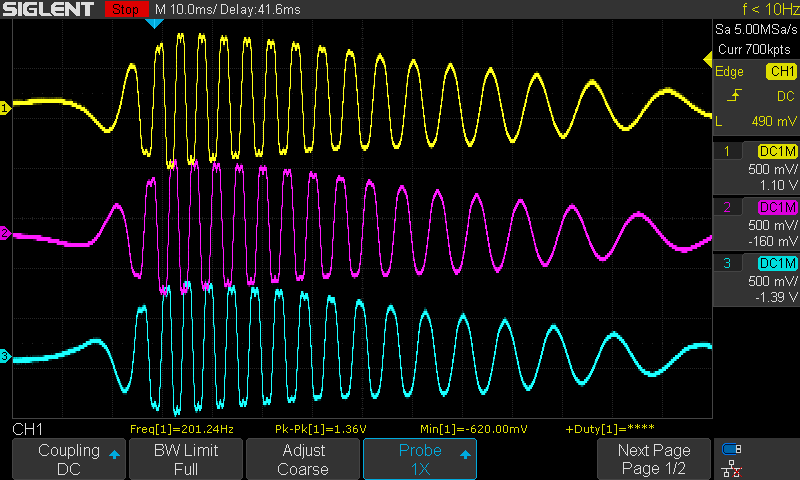
\includegraphics[width=\textwidth]{Scope/EmaxEco2306_threePhases/Freewheel/FreewheelThreePhasesGround.png}}
	\hfill
	\subfloat{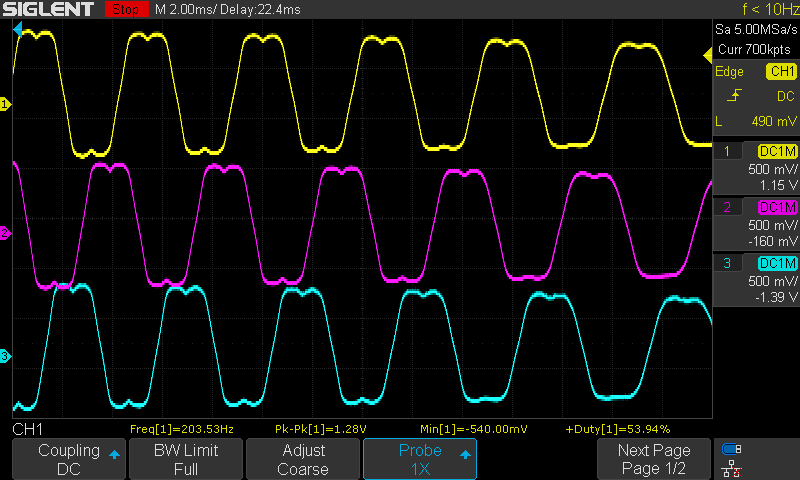
\includegraphics[width=\textwidth]{Scope/EmaxEco2306_threePhases/Freewheel/FreewheelThreePhasesGroundZoomed.png}}
	\caption{BEMF from the three phases of a used motor after spinning the rotor by hand measured with the ground rail (no battery connected) as reference}
	\label{fig:BLDC_BEMF_GND_Ref}
\end{figure}

When measuring the BEMF from the same motor but using another phase as the reference (see \autoref{fig:BLDC_BEMF_Phase_Ref_Setup}) the BEMF looks more sinusoidal as seen in \autoref{fig:BLDC_BEMF_Phase_Ref}.

\begin{figure}[H]
	\centering
	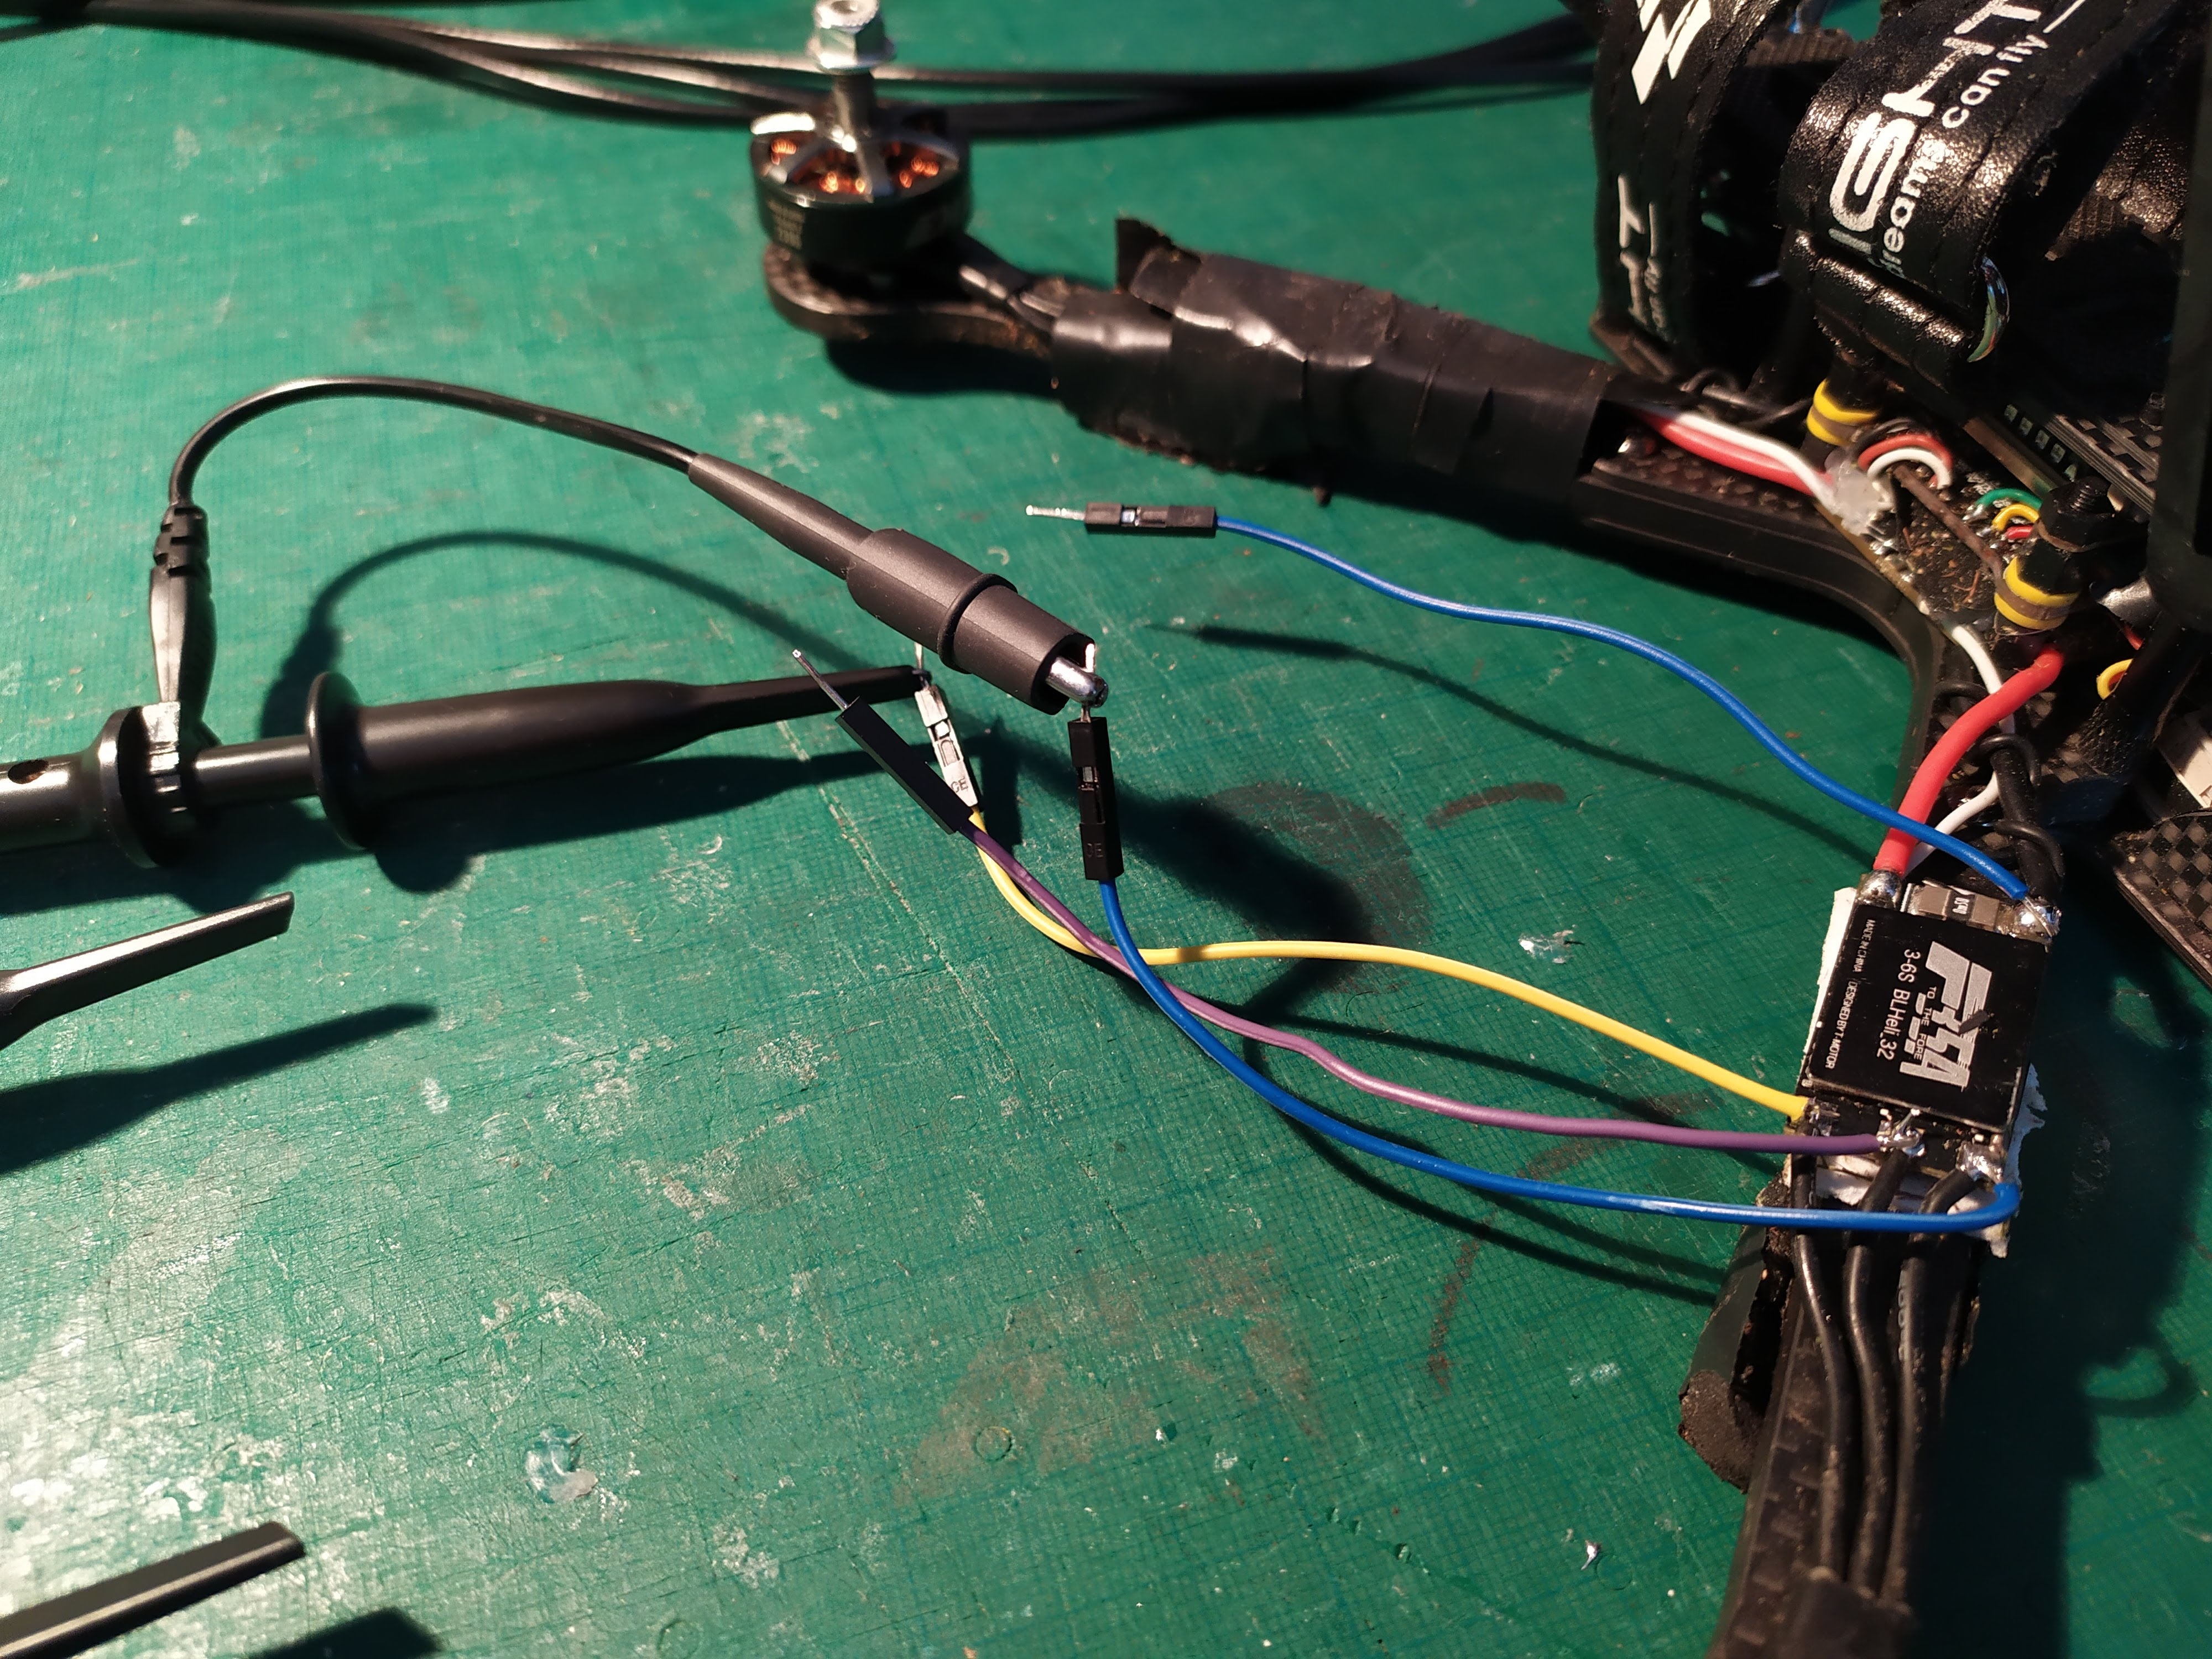
\includegraphics[width=0.75\textwidth]{Scope/EmaxEco2306_threePhases/FreeWheelSinglePhase_PhaseRef/ESC_OtherPhaseReferenceFreewheel_Setup.jpg}
	\caption{BEMF from the one phase measured with the another phase as reference. The purple wire and the blue ground wire are disconnected}
	\label{fig:BLDC_BEMF_Phase_Ref_Setup}
\end{figure} 

\begin{figure}[H]
	\centering
	\subfloat{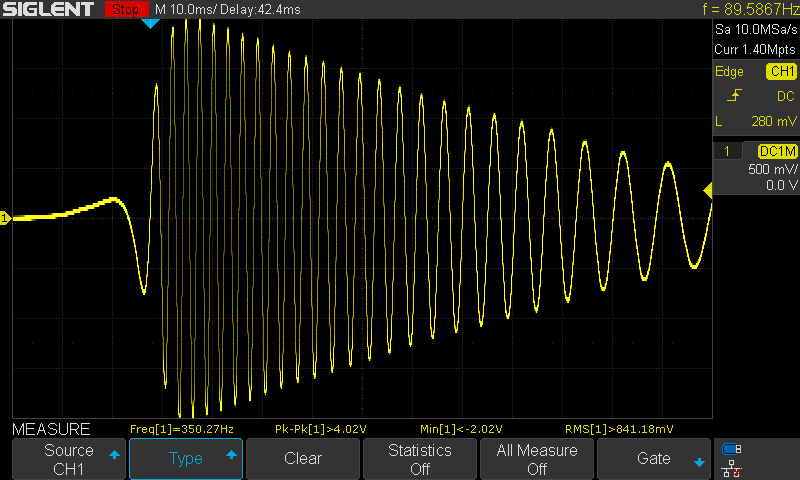
\includegraphics[width=0.49\textwidth]{Scope/EmaxEco2306_threePhases/FreeWheelSinglePhase_PhaseRef/ESC_OtherPhaseReferenceFreewheel.png}}
	\hfill
	\subfloat{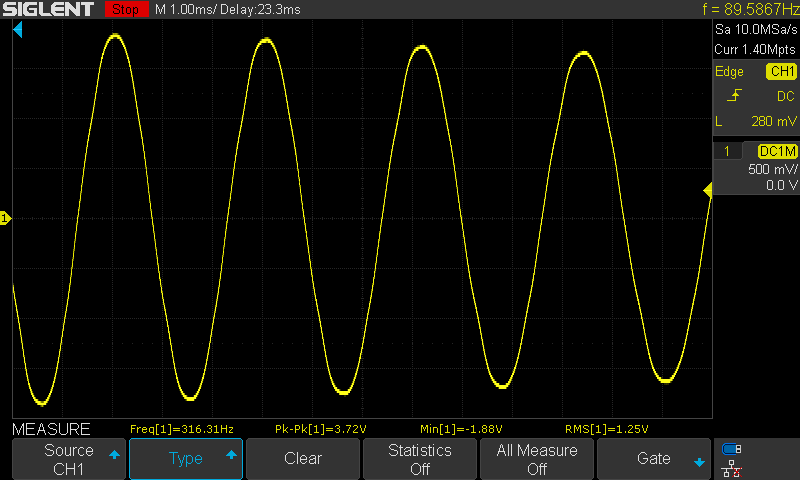
\includegraphics[width=0.49\textwidth]{Scope/EmaxEco2306_threePhases/FreeWheelSinglePhase_PhaseRef/ESC_OtherPhaseReferenceFreewheel_Zoomed.png}}
	\caption{BEMF from one phase measured with another phase as reference}
	\label{fig:BLDC_BEMF_Phase_Ref}
\end{figure}

The waveform seen in \autoref{fig:BLDC_BEMF_Phase_Ref} is simply the difference between the two phases (like you would expect) as can be shown with the math function of the oscilloscope in \autoref{fig:BLDC_BEMF_Phase_Ref_difference}. The math function is executed on waveforms similar to the ones shown in \autoref{fig:BLDC_BEMF_GND_Ref}.

\begin{figure}[H]
	\centering
	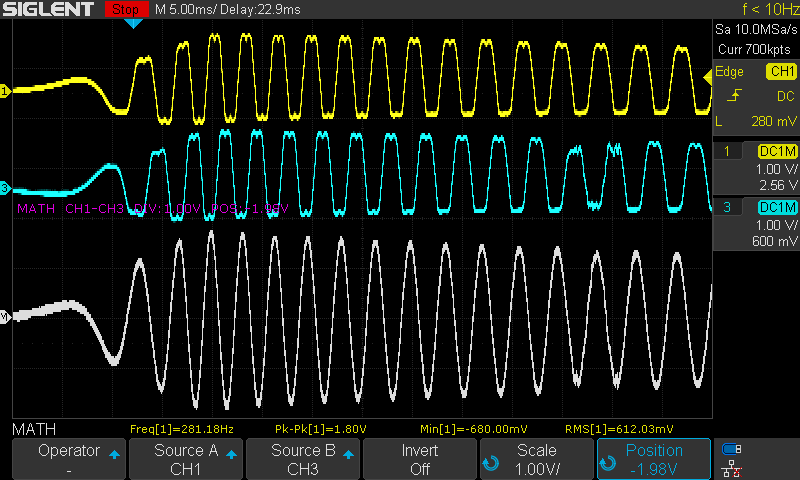
\includegraphics[width=\textwidth]{Scope/EmaxEco2306_threePhases/Freewheel/FreewheelThreePhasesGround_SubtractoinPhase1And3.png}
	\caption{Difference between phase voltages}
	\label{fig:BLDC_BEMF_Phase_Ref_difference}
\end{figure}